% !TeX encoding=utf8
% !TeX spellcheck = de-DE


\chapter{Textentnahme - es-extractor}
\chapterauthor{Mark Martinussen}

Eine der wichtigsten Anforderungen an das Projekt war eine Funktion, die den relevanten Text aus einem beliebigen Artikel zu extrahiert. In diesem Abschnitt werden wir zuerst zwei formale Ansätze betrachten und dann im Anschluss sehen wie wir diese Funktion umgesetzt haben.
% !TeX encoding=utf8
% !TeX spellcheck = de-DE
\section{Problemstellung}
Wir haben schnell festgestellt, dass es sinnvoll ist, das Extrahieren von Text nicht nur für Artikel im Internet zu betrachten, sondern für alle Websites. Zu diesem Schluss sind wir gekommen, weil das jede Website im Internet unterschiedlich aufgebaut ist und man kaum einen Artikel von einer anderen Website unterscheiden kann. Indem wir die Funktion auf beliebige Seiten des Internets ausweiten machen wir die Verwendung des Systems aus Nutzersicht einfacher, da dieser sich nicht damit befassen muss, ob eine Seite als \quote{Artikel} zählt. Weiterhin sparen wir uns aus Sicht der Entwickler und Administratoren die Notwendigkeit zu definieren welche Seiten erlaubte \quote{Artikel} sind. Insbesondere gibt es potenziell unendliche viele zulässige \quote{Artikel}, alle einzutragen oder eine Regel dafür aufzustellen wäre vermutlich unmöglich.
Im Folgenden soll Artikel gleichbedeutend mit einer beliebigen Website, die Text enthält, sein.\\
Wir definieren Text eines Artikels als relevant, wenn er einen inhaltlichen Nutzen hat. Dies sind zum Beispiel Überschriften, Unterüberschriften, inhaltlicher Text, Listen und ähnliches. Wir wollen vermeiden Teile wie Navigationselemente, Werbung, Kommentare und Verlinkungen zu extrahieren. \\
Mit dem Kontext unserer Architektur lässt sich die Aufgabe weiter konkretisieren. Die Aufgabe der Textentnahme ist es also, einen Link entgegenzunehmen und für diesen zu bestimmen, welche Teile dieser Website relevant sind. Die Architektur sollte zu der Microservice – orientierten Architektur passen, heißt, es sollte ein REST Interface geben und das Ergebnis muss so formatiert sein, dass es auch wieder gut von anderen Microservices verwendbar ist. Es dürfen somit keine prozessspezifischen Adressen, Objekte oder Datenstrukturen zurückgegeben werden. \\ \par
Soweit die Grundlagen – ein REST Interface zu implementieren ist relativ simpel und benötigt keine weitere theoretische Diskussion. Wir werden es ausschließlich im \autoref{extractor:sec:impl} über den schlussendlichen Aufbau betrachten. Viel wichtiger ist jedoch die Frage, wie wir nun bestimmen können welcher Teil einer Website relevant ist. 

% @ TODO Add "Microservice" to Glossary?

% !TeX encoding=utf8
% !TeX spellcheck = de-DE
\section{Theoretische Lösungsansätze}
\subsection[Die reduzierte Druckansicht]{Ansatz 1: Druckansicht}% \addcontentsline{toc}{subsection}{Ansatz 1: Druckansicht} % Add to table of contents without enumerating
\label{extractor:ansatz:subsec1}
Der erste Ansatz, den wir in Betracht gezogen haben, um den Inhalt eines Artikels zu extrahieren war die \quote{Druckansicht} der Seite zu verwenden. Hiermit ist diejenige Version des Artikels gemeint, welche erzeugt werden würde, wenn man mit einem Browser die Seite auf Papier ausdruckt. Wie uns aufgefallen ist, besitzen einige Seiten eine Druckansicht, die sich von der dargestellten Version unterscheiden, oft indem Elemente wie Navigation, Bilder und Werbung entfernt sind und fast nur der Inhalt dargestellt wird. Beispielsweise die News – Seite \url{www.heise.de} besitzt für all ihre Artikel eine solche Druckversion. (siehe Abb. \ref{extractor:image:druckansicht})

\begin{figure}[t]
	\centering
	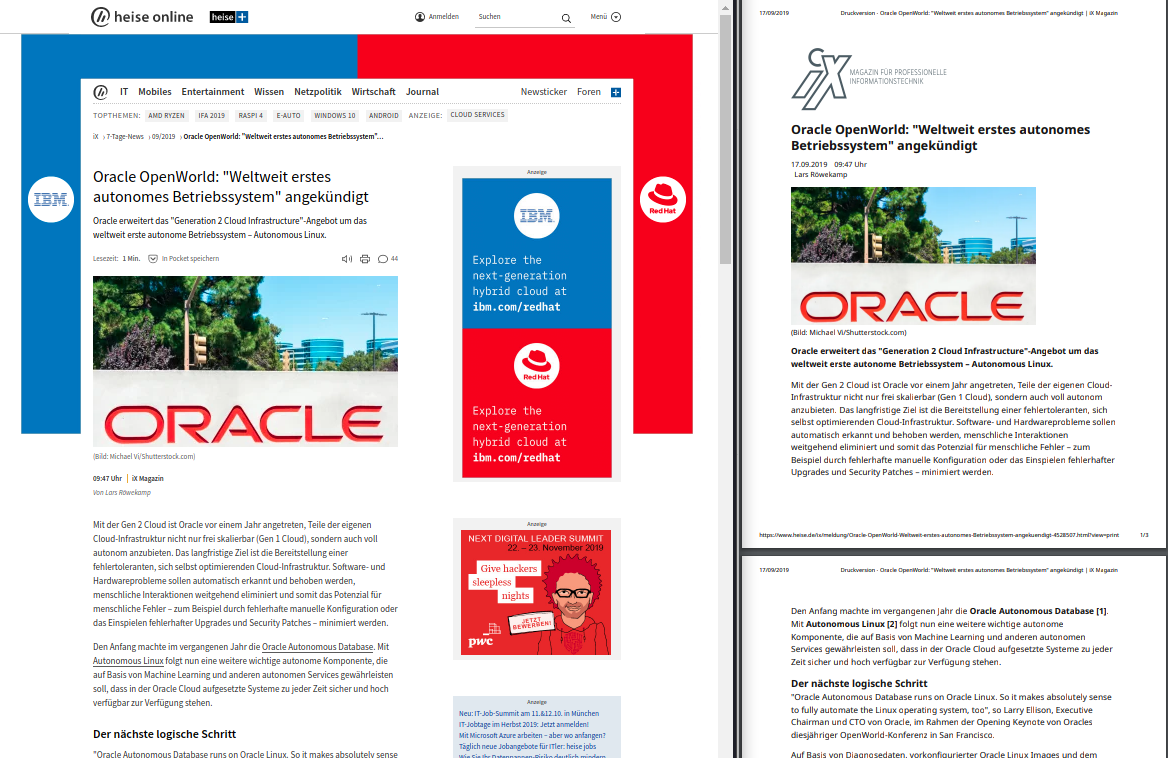
\includegraphics[width=\linewidth]{images/druckansicht.png}
	\caption{Ein Artikel und dessen reduzierte Druckversion}
	\label{extractor:image:druckansicht}
\end{figure}

Man sieht wie die vollständige Website auf der linken Seite Navigationselemente und Werbung, die wir als nicht relevant ansehen enthält. Rechts sind dahingegen nur die relevanten Inhalte zu sehen. Falls wir also in der Lage sind, zu einem solchen Artikel vom Link auf diese Druckansicht zu schließen, könnten wir diese verwenden, um den relevanten Text einer Website zu bestimmen. Um diesen Lösungsansatz zu implementieren muss man mit zwei zentralen Fragen beschäftigen.
\begin{enumerate}
	\item Wie erhält man die Druckansicht des Artikels, falls diese existiert?
	\item Kann man bestimmen ob eine Website überhaupt eine reduzierte Druckansicht hat? 
\end{enumerate}
Ein Werkzeug zur Lösung der ersten Frage sind \quote{headless} Webbrowser. Der Begriff \quote{headless} beschreibt hierbei, dass ein Programm, welches normalerweise mit einer grafischen Benutzeroberfläche ausgeführt wird, komplett ohne diese rein algorithmisch gesteuert wird. Wir werden in Abschnitt \ref{todo} sehen, wie man einen headless Browser verwendet, da wir für das Rendern von Bildern die gleiche Herausforderung haben werden. \\ \\
Aufgrund der zweiten Frage müssen wir leider feststellen, dass dieser Lösungsansatz nicht ausreichend ist. So gibt es keinen uns bekannten Weg, festzustellen ob ein Artikel eine reduzierte Druckansicht anbietet. Wie oben besprochen, ist jede Website unterschiedlich und es gibt keine fest definierte Schnittstelle. Weiterhin würde dieser Lösungsansatz eben auch nur bei Artikeln funktionieren, die eine solche Druckansicht anbieten, aber eben nicht, bei all jenen, die keine anbieten. Somit können wir unser Ziel mit diesem Ansatz nicht erreichen und müssen ihn leider verwerfen.


\subsection[HTML DOM]{Ansatz 2: HTML DOM} %\addcontentsline{toc}{subsection}{Ansatz 2: HTML DOM} 
\label{extractor:ansatz:subsec2}
Statt zu versuchen auf ein komplexes Feature, welches nur von bestimmten Seiten angeboten wird, zuzugreifen haben wir einen Ansatz entwickelt, welcher lediglich die HTML Datei einer Website benötigt. Eine jede Website wird durch eine HTML Datei beschrieben, die man ganz einfach mit dem Link herunterladen kann.
Diese Datei besitzt ein wohl definiertes Format. Die Idee dieses Ansatzes ist es nun, sich ebenjenes Format, und insbesondere die Meta – Informationen, die es enthält, zu nutzen zu machen, um den relevanten Text zu bestimmen. \\ \\ 
Der Aufbau einer HTML Datei oder HTML Dokument, wird durch das \ac{HTML DOM} beschrieben: Ein Dokument besteht aus mehreren Elementen, wobei ein Element mit den spitzen Klammern \mintinline{html}{<name>} eingeleitet und mit \mintinline{html}{</name>} terminiert wird. Im Sinne des \ac{HTML DOM} sind diese Elemente Objekte. Das heißt, sie besitzen Eigenschaften (Attribute), Methoden und Ereignisse. \cite{w3c_html} Elemente die geschachtelt definiert sind, bilden eine Vererbungsbeziehung, wobei das oberste Objekt immer \verb|document| genannt wird. Ein HTML Dokument beschreibt einen Baum (Abbildung \ref{extractor:image:html}), mit einem \verb|head| für Metainformationen und einem \verb|body| für den Inhalt. Dieser Inhalt kann dann weiter in Absätze, Überschriften, usw. unterteilt sein.  
\begin{wrapfigure}{r}{0.4\textwidth}
	\centering
	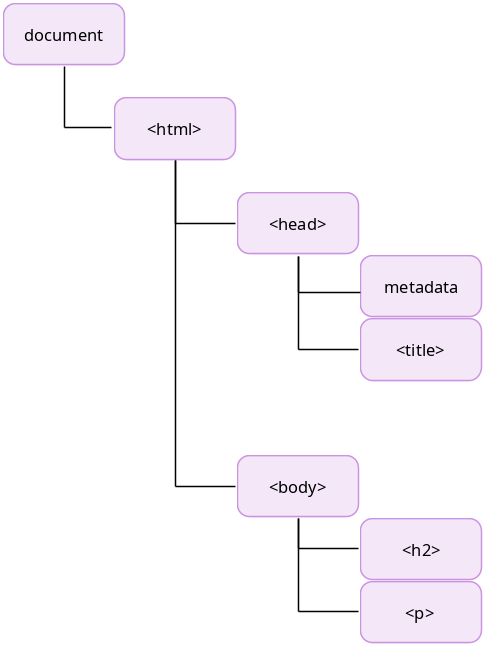
\includegraphics[scale=0.7]{images/html_overview.png}	
	\caption{Struktur eines HTML Dokumentes}
	\label{extractor:image:html}
\end{wrapfigure}

Nun können wir die Eigenschaften dieser Objekte auszunutzen. Beispielsweise gibt es das Attribut \mintinline{js}{document.body.textContent}, das allen angezeigten Text des Artikels enthält. Dieses beinhaltet jedoch auch den Text der Navigationselemente und Werbung. Folglich ist dieses Attribut alleine nicht ausreichend.

\subsubsection*{CSS Query Selectors}
Zusätzlich zu seinen Attributen kann ein Element auch mit einer Klasse und einer ID dekoriert werden. Diese sind nicht direkt Teil von HTML, aber stattdessen Teil des CSS Stylings. So kann ein Webentwickler bestimmen, dass der Absatz, der den Haupttext enthält, eine bestimmte ID hat oder Teil einer Klasse ist. IDs, Klassen und HTML Elemente können dann mit sogenannten CSS Query Selectors abgefragt werden. Diesen Umstand können wir uns zunutze machen und selber diese Selektoren ausführen, um an die gewünschten Elemente zu kommen. Ein Auszug aus der Syntax Definition:
\begin{itemize}
	\item \mintinline{html}{element element2} Wählt alle Elemente aus, deren Vorfahre ein HTML Element \quote{element} ist, und die selber ein Element vom Typ \quote{element2} sind.
	\item \mintinline{html}{element,element2} Wählt Elemente aus, die entweder element oder element2 sind.
	\item \mintinline{html}{.class} Wählt alle Elemente aus, deren Klasse \quote{class} ist.
	\item \mintinline{html}{#id} Wählt alle Elemente aus, deren ID gleich \quote{id} ist.
	\item \mintinline{html}{[attribut]} Wählt alle Elemente aus, die ein solche Atrribut besitzen.
\end{itemize}
Nun sind wir in der Lage, diese Query Selectors anzuwenden um den relevanten Text eines Artikels zu bestimmen. Beispielsweise können wir mit der Zeile 
\begin{minted}{js}
document.body.querySelectorAll(
	'.a-article-header__title,.a-article-header__lead,.article-content')
\end{minted}
die relevanten HTML ELemente eines beliebigen Artikels von \url{www.heise.de} extrahieren. Die Formatierung bleibt hierbei erhalten, heißt wir können sogar Überschriften, Zitate, Aufzählungen und Tabellen unterscheiden und später unverändert anzeigen. Um den reinen relevanten Text zu erhalten würden wir von jedem Listenelement das \verb|textContent| Attribut verwenden.
























% !TeX encoding=utf8
% !TeX spellcheck = de-DE
\section{Mercury Parser API}
Wie wir in Abschnitt \ref{extractor:ansatz:subsec2} besprochen haben, können wir mithilfe des \ac{HTML DOM} und CSS Query Selectors zuverlässig den relevanten Text  eines Artikels bestimmen. Damit wir nicht Selektoren für alle Websites der Welt definieren müssen, verwenden wir eine Library, die uns viel Arbeit abnimmt. Der Mercury Web Parser von Postlight Labs LLC\cite{mercury_homepage} verwendet genau eine Menge von komplexen CSS Query Selectors und Eigenschaften des HTML DOM um für einen beliebigen Artikel den relevanten Text und mehr zu bestimmen. Der Mercury Parser kann mit nur einer URL oder zusätzlich dem schon heruntergeladenen HTML Dokument aufgerufen werden. In der Praxis verwenden rufen wir ihn nur mit der URL auf. Zusätzlich definieren wir den HTTP Header der Anfrage und mit welcher Formatierung (keine, HTML, Markdown) der relevante Text extrahiert werden soll.
% @TODO Uncomment, for some reason putting minted inside a listing to include a caption causes bugs.
%\begin{listing}[ht]
%	\label{extractor:code:mercury}
%	\caption{Beispielhafter Aufruf des Mercury Web Parsers}
	\inputminted[
		frame=lines, 
		framesep=2mm, 
		linenos, 
		baselinestretch=1.2, 
		fontsize=\footnotesize]{js}{code/mercury-example.js}
%\end{listing}


\begin{center}
\textuparrow\textcolor{blue}{@TODO: Uncomment the listing!} \textuparrow
\end{center}


Das Ergebnis ist ein \ac{JSON} Objekt, die enthaltenen Felder sind in Tabelle \ref{extractor:table:mercury} aufgelistet. Falls der Parser den Wert für ein Feld nicht bestimmen kann, ist er \verb|null|.
\begin{table}[t]
	\centering
	\begin{tabu}{lX}
		\toprule
		Feld & Beschreibung \\ \midrule
		\texttt{title} & Titel oder Überschrift der Website. \\
		\texttt{content} & (Formatierter) Text, welcher als relevant angesehen wird. Mögliche Formate sind HTML, Markdown oder keins. \\
		\texttt{author} & Autor oder Editor der Seite / Artikels. \\
		\texttt{date\_published} & Zeitpunkt zu dem die Website veröffentlicht wurde. \\
		\texttt{lead\_image\_url} & URL des Vorschaubildes.  \\
		\texttt{dek} & Abstrakte Zusammenfassung des Artikels, die unter dem Titel steht. \\
		\texttt{excerpt} & Ein kleiner Ausschnitt des Artikels, oft die ersten paar Sätze oder identisch mit dem \texttt{dek}. \\
		\texttt{total\_pages} & Anzahl der Seiten (HTML Dokumente) über die sich dieser Artikel erstreckt.\\
		\texttt{next\_page\_url} & URL der nächsten Seite (HTML Dokument) des Artikels, falls der Artikel aus mehreren Seiten besteht. \\
		\texttt{rendered\_pages} & Anzahl der Seite (HTML Dokumente), die betrachtet wurden. \\
		\texttt{url} & URL der Website. \\
		\texttt{domain} & Domain der Website. \\
		\texttt{word\_count} & Anzahl der Wörter im relevanten Text auf der Seite. \\
		\texttt{direction} & Vermutete Leserichtung des Artikels. Meistens \quote{ltr} oder \quote{rtl}. \\ \bottomrule
		
	\end{tabu}
\caption{Rückgabewerte des Mercury Web Parsers}
\label{extractor:table:mercury}
\end{table}

\subsection{Benutzerdefinierte Selektoren}
Trotz der fortlaufenden Arbeit, die an dem Mercury Web Parser gemacht wird, haben wir feststellen müssen, dass er bei weitem nicht perfekt ist. Insbesondere, da er von einem englischsprachigen Team entwickelt wird, werden deutschsprachige Websites und Artikel oft nur unzureichend analysiert. Eine HTML Datei mit deutschen IDs und Klassen wie \verb|.mitte| oder \verb|#inhalt| ist für den Parser unverständlich. Glücklicherweise sind die Entwickler sich dieses Problems bewusst und bieten eine Lösung an. \\
Es gibt die Möglichkeit, für eine Domain die unzureichend erkannt wird, benutzerdefinierte Selektoren anzulegen. Intern heißen diese \quote{Extraktoren}, wir werden diesen Begriff jedoch nicht verwenden, um Missverständnisse vorzubeugen. Bei diesen Selektoren handelt es sich ein \ac{JSON} Dokument, bei dem jedem Feld eine Menge von CSS Query Selectors zugeordnet wird. \cite{mercury_custom} Beispielsweise ein benutzerdefinierter Selektor für die deutsche News – Seite \url{www.golem.de}.

\inputminted[
frame=lines, 
framesep=2mm, 
linenos, 
baselinestretch=1.1, 
fontsize=\footnotesize]{js}{code/golemextractor.js}
% @TODO Caption.















% !TeX encoding=utf8
% !TeX spellcheck = de-DE
\section{Implementierung} \label{extractor:sec:impl}
Mit dem Mercury Web Parser sind wir in der Lage zuverlässig den relevanten Text eines Artikels zu extrahieren.
Deshalb ist der \hyperref{https://github.com/elastifeed/es-extractor/}{}{}{es-extractor} wenig mehr als ein Wrapper für den Mercury Web Parser, der dessen Funktionen als REST Interface zur Verfügung stellt. Der es-extractor ist komplett mittels JavaScript's \mintinline{js}{async/await} Syntax zur asynchronen Programmierung implementiert. Dies bedeutet, dass verschiedene Aufgaben gleichzeitig abgearbeitet werden können. Beispielsweise muss eine zweite Anfrage nicht darauf warten, dass die Seite der ersten Anfrage geladen ist, bevor sie selber anfangen kann, zu laden. In unseren Tests können 2 bis 3 Anfragen gleichzeitig bearbeitet werden, ohne dass es zu spürbaren Leistungsverlusten kommt. \par
Eine erfolgreiche Abarbeitung einer Anfrage resultiert in einer HTTP 1.1 Antwort mit dem Statuscode 200. \verb|Content-Type| ist \verb|application/json|, mit UTF-8 Zeichenkodierung. Das Datum ist ein \ac{JSON} Objekt, welches dieselben Felder enthält wie die Antwort des Mercury Web Parser (Tabelle \ref{extractor:table:mercury}), mit Ausnahme des \verb|content| Feldes. Das \verb|content| Feld ist durch 2 Felder ersetzt worden: \\ \\
	\begin{tabu}{lX}
		\toprule
		Feld & Beschreibung \\ \midrule
		\texttt{raw\_content} & Relevanter Text des Artikels, komplett ohne Textformatierung. Dieses Feld sollte genutzt werden um Suchanfragen und ähnliches zu starten. \\
		\midrule
		\texttt{markdown\_content} & Relevanter Text, der als Markdown \cite{markdown2016} formatiert ist. Dieses Feld sollte verwendet werden, um den Text anzuzeigen, da er die ursprüngliche Form des Artikels beibehält. Er kann auch Links zu Bildern enthalten, die heruntergeladen werden müssen. \\
		\bottomrule
	\end{tabu}
\subsection{Schnittstellen}
Bei Programmstart wird standardmäßig ein HTTP Server auf \verb|http://localhost/|, Port 8080 gestartet. Dieser stellt 2 Endpunkte zu Verfügung, die beide nur auf einen HTTP 1.1 POST Request mit \verb|Content-Type: application/json| reagieren. 
\paragraph{/mercury/url} Dieser Endpunkt erwartet ein \ac{JSON} Objekt mit einem \quote{url} Feld. Die URL muss die URL der Website sein, von der der relevante Text bestimmt werden soll.
\mint{json}{{"url" : "http://example.com"}}
\paragraph{/mercury/html} Dieser Endpunkt erwartet ein \ac{JSON} Objekt mit einem \quote{url} Feld und einem \quote{html} Feld. Die URL muss die URL der Website sein, von der der relevante Text bestimmt werden soll und das HTML Feld muss dessen komplettes HTML enthalten.
\begin{minted}{json}
{
 "url"  : "http://example.com" , 
 "html" : "<html><head><title>Example<\title>..."
}
\end{minted}
\subsection{Logging}
Der es-extractor besitzt grundlegende Protokollierung, die zu \verb|stdout| geschrieben werden. Der Logger basiert auf dem \hyperref{https://www.npmjs.com/package/winston}{}{}{Winston Logger} für NPM, man kann ihm einen neuen \quote{Transport} hinzuzufügen, um dafür zu sorgen, dass die Protokolle von außen erreichbar sind. \\ 
Die Ausgabe enthält immer zuerst das Log - Level (info, warn, error), den Tag und die Uhrzeit. Eine Ausgabe, die durch eine Anfrage an den Server erzeugt wurde, beinhaltet zusätzlich eine ID, die diese Anfrage eindeutig identifiziert. Schlussendlich kommt die Nachricht.
\subsection{Fehlermeldungen}
Falls es während der Laufzeit zu einem Fehler kommt, wird dieser Fehler zuerst mit einem entsprechenden Level protokolliert. Eine Anfrage die einen Fehler erzeugt, bekommt grundsätzlich immer eine HTTP 1.1 Antwort mit einem Statuscode der ungleich 200 ist. In Fällen wo der Fehler beispielsweise durch eine inkorrete URL oder HTML Dokument erzeugt wird, wird zusätzlich ein JSON Dokument mit einer Nachricht zurückgeschickt.





















\chapter{Rendern von Websites - es-scraper}
\chapterauthor{Mark Martinussen}

In diesem Abschnitt werden wir sehen, wie wir aus einer HTML Datei PDF und JPG Dateien generieren können. Zusätzlich besprechen wir, wie wir diese rechenintensiven Aufgaben so effektiv wie möglich bearbeiten können, was uns dann schließlich zu der Implementierung des es-scraper bringen wird. 
% !TeX encoding=utf8
% !TeX spellcheck = de-DE
\section{Problemstellung}
Ergänzend zum Auslesen des relevanten Textes einer Website muss diese ebenfalls in Bildform angezeigt werden. Speziell wurde definiert, dass jede Seite in Form einer PDF und eines Screenshots vorlegen muss. \\
Dazu müssen wir bestimmen, wie man eine HTML Datei in solche Formate umwandelt. Wie benötigen also eine Art HTML Parser. Am bekanntesten sind HTML Parser in Webbrowsern, wo sie jeden Tag zum Einsatz kommen. Es stellt sich also die Frage, ob es einen Webbrowser gibt, der ohne eine grafische Benutzeroberfläche komplett über eine API oder als Library steuerbar ist.
Weiter haben wir bedacht, dass diese Operationen rechenintensiv sind. Demnach müssen wir einen Weg finden, die Implementierung möglichst effizient und nebenläufig zu machen. Das System darf auch bei einigen duzend Anfragen nicht hoffnungslos überlastet sein. \\
Selbstverständlich muss die Implementierung auch zu der Infrastruktur passen. Dementsprechend wird wieder ein REST Interface benötigt, die Applikation sollte nach der Philosophie der Microservices konzipiert sein und die Rückgabewerte sollten klar und einfach weiterzuverwenden sein.
% !TeX encoding=utf8
% !TeX spellcheck = de-DE
\section{Headless Webbrowser} \label{scraper:sec:headless}
Um ein HTML Dokument in eine PDF oder einen Screenshot umzuwandeln benötigen wir einen HTML Parser, der identisch zu einem Webbrowser arbeitet. So können wir sicherstellen, dass die archivierten Versionen, die wir den Benutzern anbieten mit den Originalen übereinstimmen. Dies beinhaltet nicht nur das Anzeigen von HTML, sondern auch das Ausführen von Javascript, Herunterladen von externen Bildern und ähnlichen Elementen sowie Anordnung aller Komponenten zu einem ganzen. \\
In dem Webbrowser Google Chrome gibt es die Möglichkeit eine Seite zu \quote{Inspizieren} (siehe Abbildung \ref{scraper:image:cdpinspect}). Dieses Instrument erlaubt dem Nutzer den Seiten zu bearbeiten und Probleme zu diagnostizieren. Intern heißen sie die Chrome DevTools. Mit einer langen Liste von Funktionen kann man sagen, dass die Chrome DevTools in der Lage sind, einen Webbrowser komplett zu emulieren:
\begin{itemize}
	\item Zugriff auf den HTML – Renderer von Chrome
	\item Sichtung und Modifikation des \ac{HTML DOM}
	\item Simulieren beliebiger Endgeräte
	\item Ausführung und Testen von Javascript
	\item Prüfen der Netzwerkaktivität
	\item Zugriff zu Cookies, Arbeitsspeicher und Websiteinterne Ressourcen
\end{itemize}


\begin{figure}[h]
	\centering
	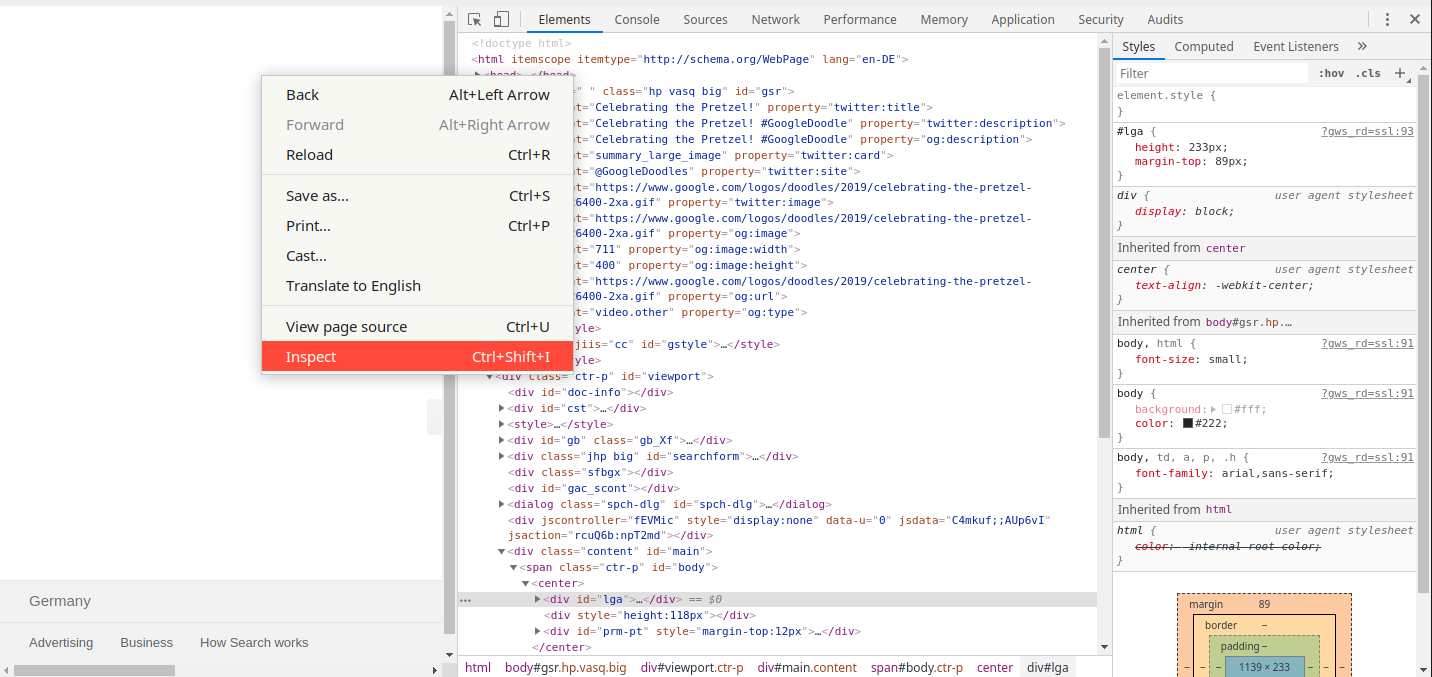
\includegraphics[width=\linewidth]{images/cdp_inspect.png}
	\caption{Zugriff auf die Chrome DevTools in Google Chrome}
	\label{scraper:image:cdpinspect}
\end{figure}

Am wichtigsten für unseren Nutzen existiert zusätzlich eine Schnittstelle, mit dem man diese DevTools algorithmisch steuern kann. Das sogenannte \ac{CDP} ermöglicht kompletten Zugriff auf die Funktionen des Google Chrome Webbrowsers sowie des Chrome DevTools. Das \ac{CDP} stellt viele hundert Funktionen zur Verfügung die auf komplexe Weise zusammenarbeiten. \cite{cdpexplorer} 

\begin{figure}[h]
	\centering
	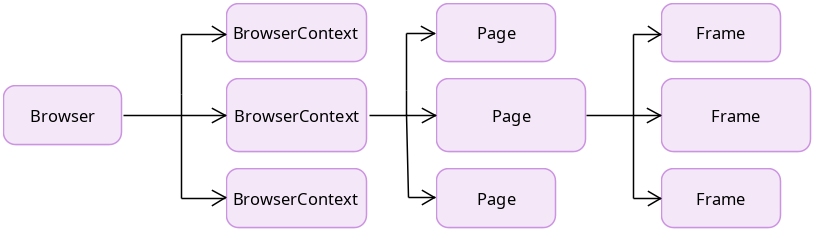
\includegraphics[]{images/cdp_overview.png}
	\caption{Struktur einer Chrome – Instanz}
	\label{scraper:image:cdptree}
\end{figure}
Abbildung \ref{scraper:image:cdptree} zeigt die Struktur einer Chrome Instanz. Das \quote{Browser} Element kann man sich als den übergeordneten Prozess vorstellen. Manchmal wird dieser auch der \quote{Allocator} genannt. Dieser Prozess besitzt dann etliche Ausführungskontexte, die größtenteils voneinander getrennt arbeiten können. Auf einem abstrakten Level kann man sie sich als verschiedene Fenster des Browsers vorstellen. Ein \quote{Fenster} hat, kann dann im Sinne von Tabs mehr als eine Seite anzeigen, welche selbst aus mindestens einem HTML Frame bestehen. \\
Wenn man mit dem \ac{CDP} entwickelt, ist es nützlich diese Struktur im Hinterkopf zu behalten. Man sollte wissen auf welcher Ebenen sich ein Funktionsaufruf auswirkt. Insbesondere können Aufrufe auch den Baum nach oben traversieren. Beispielsweise wenn ein man einen Mausklick auf einen Link im Frame simuliert, wirkt sich dieser selbstverständlich auch auf die Page aus.

%\pagebreak


Das \ac*{CDP} ist selbst in Javascript implementiert, Google empfiehlt dem normalen Entwickler es nicht direkt zu verwenden. \cite{dontuse} Für eine kleine Anwendung alle nötigen Funktionen korrekt zu verwenden sei schwer und fehleranfällig. Um auch nur einen simplen Webbrowser zu starten und zu navigieren müssen die richtigen Methoden in der richtigen Reihenfolge aufgerufen werden. Zuerst muss ein Browser erstellt oder das \ac{CDP} mit einem bestehenden Browser verbunden werden. Daraufhin müssen alle benötigten Kontexte korrekt konfiguriert werden, sodass eine Seite erstellt und navigiert werden kann. \\
Stattdessen wird geraten, vorbereitete Libraries zu verwenden, die diese komplexe Struktur abstrahieren und für die meisten Use – Cases ausreichend sind. 
\begin{table}[h]
	\centering
	\begin{tabu}{ll} \toprule
		Programmiersprache & Library \\ \midrule
		Node.js & Google Chrome Puppeteer \\
		Java & cdp4j \\
		Python & pychrome \\
		Go & chromedp, cdproto \\
		\bottomrule
	\end{tabu}
	\caption{Implementierungen des CDP}
	\label{scraper:table:cdpimpl}
\end{table}


Die obige Tabelle zeigt eine unvollständige Liste von Implementierung, die man in verschiedenen Programmiersprachen verwenden kann, um das CDP zu steuern. Wir zwei von diesen Libraries betrachten, wie wir sie verwenden können, welche Features sie bieten sowie einige Eigenartigkeiten, die uns im Projektverlauf aufgefallen sind.

\subsection*{Google Chrome Puppeteer} \label{scraper:subsec:puppeteer}
Google selbst schlägt als Abstraktion des \ac{CDP} die Verwendung ihrer eigenen Library vor. Google Chrome Puppeteer, kurz Puppeteer, ist eine Node.js API, welche die meisten Funktionen des \ac{CDP} implementiert um eine Chrome Instanz headless, oder mit einer Benutzeroberfläche zu steuern. \cite{puppeteer} Im Vergleich zur Verwendung des reinen \ac{CDP} ist Puppeteer einfach. So können wir einen neuen headless Browser starten und eine Website mit nur wenigen Zeilen laden.
\begin{minted}[frame=lines, 
framesep=2mm, 
linenos, 
baselinestretch=1.2, 
fontsize=\footnotesize]{js}
const puppeteer = require('puppeteer');

// Start a browser
const browser = await browser.launch(); 
// Create a page in the default context of this browser.
const page = await browser.newPage();  
// Navigate to a page
await page.goto('http://example.com/'); 
\end{minted}
In Hinblick auf Abbildung \ref{scraper:image:cdptree} ist auffällig, dass anscheinend kein BrowserContext erstellt werden muss. Es scheint, als ob eine Seite direkt in dem Hauptprozess / Allocator erstellt werden kann. Die ist jedoch nicht der Fall. Die Dokumentation von Puppeteer spezifiziert, dass alle Seiten in einem Standard – BrowserContext erstellt werden. Es ist zwar möglich mit der Funktion \mintinline{js}{browser.createIncognitoBrowserContext()} einen zusätzlichen Kontext anzulegen, dieser teilt aber keine Informationen mit den anderen Kontexten. Für besondere Fälle kann dies zu einem Problem werden und erfordert, dass man direkt mit dem CDP kommuniziert, um einen weiteren Kontext zu erstellen. Beispielsweise kann es sein, dass man in zwei Kontexten auf der gleichen Seite arbeiten möchte. Dies hat den Vorteil, dass man beide Kontexte parallel bearbeiten kann, während Informationen wie Cookies mit Login Daten zwischen den Kontexten geteilt werden. \footnote{Dies ist uns in der Implementierung passiert, da wir PDFs und Screenshots parallel rendern wollten.} \\
Nun können wir den HTML Renderer von Google Chrome nutzen um Screenshots und PDF Dateien herzustellen:  
\begin{minted}[frame=lines, 
framesep=2mm, 
linenos, 
baselinestretch=1.2, 
fontsize=\footnotesize]{js}
await page.screenshot({path : 'example.png'});
await page.pdf({path : 'example.pdf'});
\end{minted}
% !TeX encoding=utf8
% !TeX spellcheck = de-DE
\section{Entwicklung mit CDP in Go} \label{scraper:sec:chromedp}
Trotz der Zuverlässigkeit und Übersichtlichkeit von Google Chrome’s Puppeteer haben wir uns gegen die Verwendung dieser Library entschieden. Einerseits hatten wir keinen Entwickler im Team, der erfahren genug in der Verwendung von Node.js waren, um eine performante und stabile Implementierung zu entwickeln. Weiterhin haben wir in unseren ersten Tests Probleme mit der Nebenläufigkeit von Puppeteer gehabt. Wir konnten keinen Weg finden zuverlässig Screenshots und PDF Dateien einer Website gleichzeitig zu generieren. Da wir einen großen Fokus auf die Effizienz und Skalierbarkeit unserer Microservices legen, sind wir nicht in der Lage diese Library zu verwenden, obwohl es vermutlich die einfachste Variante ist. \\ \\
Die Programmiersprache Go bietet mächtige Primitive zur Entwicklung performanter, nebenläufiger Anwendungen. Es existiert ebenfalls eine direkte Implementierung des CDP in Go, bekannt als das Paket cdproto. Diese Library enthält generierten Code für alle des CDP definierten Befehle wie sie auch in der Referenzimplementierung zur Verfügung stehen. Diese Befehle zu generieren ist möglich, da das CDP nicht nur in Javascript implementiert ist, sondern auch vollständig mit PDL (Program Design Language) beschrieben ist. Aus dieser beschreibenden Sprache kann dann Quellcode für beliebige Programmiersprachen generiert werden.  \cite{https://github.com/chromedp/cdproto-gen}
Die Verwendung dieser Library ist immer noch sehr komplex. Auf der Grundlage des Pakets cdproto wird dann die Library chromedp entwickelt. Diese abstrahiert, ähnlich wie Puppeteer, die komplexen Funktionalitäten und vereinfacht die Nutzung. Ein großer Vorteil von der Implementierung in Go, dass die Standardbibliothek Kontexte ausgezeichnet unterstützt. \cite{go_context} Dadurch wird die Abbildung der Struktur einer Chrome Instanz sehr gut verwirklicht. Die Funktion \mint{go}{func NewContext(parent context.Context, opts ...ContextOption)} 
erstellt so je, nachdem mit welchem Vorgänger sie aufgerufen wird, einen Browser mit einem BrowserContext und einer Page oder einen BrowserContext mit einer Page in einem bestehenden Browser oder eine lediglich einen weiteren \quote{Tab} im selben BrowserContext.
\begin{listing}[h]
	\inputminted[
	frame=lines, 
	framesep=2mm, 
	linenos, 
	baselinestretch=1.2, 
	fontsize=\footnotesize]{go}{code/chromedp_context_1.go}
	\caption{Erstellung von geschachtelten Kontexten mit chromedp}
	\label{scraper:code:chromedpctx}
\end{listing}

\begin{listing}[h]
	\inputminted[
	frame=lines, 
	framesep=2mm, 
	linenos, 
	baselinestretch=1.2, 
	fontsize=\footnotesize]{go}{code/chromedp_context_2.go}
	\caption{Verwendung der Allocatorfunktionen in chromedp}
	\label{scraper:code:chromedpalloc}
\end{listing}

Wenn wir mehr Kontrolle über die Struktur unseres Browsers wünschen, können wir mit der Funktion \mint{go}{func NewExecAllocator(parent context.Context, opts ...ExecAllocatorOption)} nur den Allocator, also den Hauptprozess des Browsers, erzeugen. Mit diesem als Basis können wir nun beliebig viele BrowserContexts und Pages erstellen indem wir wieder die Funktion \mintinline{go}{chromedp.NewContext(...)} verwenden. 


In dem Beispiel \ref{scraper:code:chromedpalloc} erschaffen wir nun also Schrittweise zuerst den Hauptprozess, dann zwei BrowserContext, welche man als \quote{Browser Fenster} verstehen kann. Gefolgt davon erzeugen wir 2 Tabs im ersten Fenster und einen Tab im zweiten Fenster. Wichtig ist, dass bei jedem Aufruf von \mintinline{go}{chromedp.NewContext(...)} immer ein Standardtab erzeugt wird, der Aktionen ausführen kann. Deshalb besitzen wir in Listing \ref{scraper:code:chromedpalloc} zwei Tabs mehr. Unsere Empfehlung ist, diese der Verständlichkeit wegen zu ignorieren. 

Um eine Aktion auf mit einem Tab auszuführen, dient die \\
\mintinline{go}{chromedp.Run(ctx context.Context, actions ...Action)} Funktion, die eine Liste von Aktionen auf einem Kontext ausführt. 
\begin{minted}[
frame=lines, 
framesep=2mm, 
linenos, 
baselinestretch=1.2, 
fontsize=\footnotesize]{js}
tasks := chromedp.Tasks{
  chromedp.Navigate("http://example.com"),
  chromedp.CaptureScreenshot(&result)
}
chromedp.Run(tab1_1, tasks)
\end{minted}
\pagebreak
\subsection{Verbindung zu einem bestehenden Browser} \label{scraper:subsec:go:remote}
Das CDP ermöglicht nicht nur die Erzeugung eines neuen Webbrowsers, sondern kann sich auch an einen bestehenden Browser verbinden. Dies hat den großen Vorteil, dass es zwischen verschiedenen Systemen keine unerwarteten Probleme gibt, wenn verschiedene Versionen von Chrome, den CDP und Go verwendet werden. Beispielsweise kann man einen Chrome Browser in einem Docker Container ausführen und so sicherstellen, dass auf allen Systeme derselbe Browser läuft. Die Funktion \mint{go}{func NewRemoteAllocator(parent context.Context, url string)} verbindet das CDP in Go mit einem beliebigen Chrome Instanz an einer Url. Es wird dann eine Verbindung über das Websocket Protokoll hergestellt. Damit sich das CDP an eine Browser Instanz verbinden kann, muss diese den entsprechenden Port öffnen. Mit dem Aufruf \mint{bash}{chrome --headless --remote-debuggig-port=9222} wird ein headless Browser gestartet, an den sich das CDP über  \verb|ws://localhost:9222| verbinden kann.

\subsection{Navigieren von Tabs} \label{scraper:subsec:go:navigate}
Um eine Funktion aus der chromedp Library, die nicht ausreichend oder fehlend ist, zu ersetzen verwendet man den Typ \mintinline{go}{type ActionFunc func(context.Context) error}, um eine herkömmliche Funktion in einem Kontext ausführbar zu machen. So haben wir die Navigation mit den Funktionen aus cdproto neu definiert, um sie an unseren Nutzen anzupassen.

\begin{listing}[h]
	\inputminted[
	frame=lines, 
	framesep=2mm, 
	linenos, 
	baselinestretch=1.2, 
	fontsize=\footnotesize]{go}{code/chromedp_navigate.go}
	\caption{Neudefinition der Navigation in chromedp}
	\label{scraper:code:navigate}
\end{listing}
Zuerst verwenden wir das \verb|emulation| Modul des CDP, um sicherzustellen, dass der User Agent gesetzt ist. Ohne User Agent bekommen wir keinen Zugang zu manchen Websites, die Beispielsweise erwarten, dass ein Nutzer zuerst den Cookies zustimmt, bevor man weitergeleitet wird. Daraufhin navigieren wir den Tab und warten darauf, dass ein \verb|PageLoadEvent| ankommt. Dieses Event signalisiert, dass die Website vollständig geladen ist und der Tab ihren gesamten Inhalt anzeigt. Wenn zu viele Seiten parallel geladen werden, kann es zu einem Data Race kommen. Dies liegt daran, dass der Browser mehrere \verb|PageLoadEvent|s gleichzeitig erhalten würde, aber immer nur eins davon an das CDP weitersenden kann. Dadurch würden gelegentlich Tabs unendlich auf ihr \verb|PageLoadEvent| warten. Um dies zu vermeiden haben wir ein einminütiges Timeout definiert, nach welchem wir annehmen, dass eine Seite geladen ist. \\ Schlussendlich speichern wir die vollständige Größe des gesamten Inhalts der Website ab. Dies ist nützlich, damit wir wissen, wie groß der Screenshot und die PDF sein müssen. Der Rückgabewert ist immer \verb|nil|, es sei den, bei der Navigation ist ein Fehler aufgetreten.

\subsection{Generierung von PDFs} \label{scraper:subsec:go:pdf}
Das Generieren von PDF Dateien nutzt die Druckansicht der Website. Effektiv wird also nur ein \quote{Rechtsklick > Drucken} simuliert. Diese Funktion ist Teil des Chrome Browsers und somit über das CDP Aufrufbar.  
\begin{listing}[h]
	\inputminted[
	frame=lines, 
	framesep=2mm, 
	linenos, 
	baselinestretch=1.2, 
	fontsize=\footnotesize]{go}{code/chromedp_pdf.go}
	\caption{Generieren von PDF Dateien}
	\label{scraper:code:pdf}
\end{listing}
Als einzige zusätzlich Aktion wird vorher die \verb|setDeviceMetricsAction| aufgerufen. Diese Funktion dient dem Zweck, die Maße des Tabs auf die Größe des gesamten Inhalts zu setzen, welche während der Navigation bestimmt worden war. Dies stellt sicher, dass die ganze Seite dargestellt wird. Das Ergebnis der \verb|PrintToPDF| Funktion ist die PDF, codiert in Base64. Wie diese Daten abgespeichert werden, besprechen wir in Abschnitt \ref{todo}.
\subsection{Generierung von Screenshots} \label{scraper:subsec:go:screenshot}
Um einen Screenshot zu Erstellen, benutzen wir den HTML Renderer von Chrome. Wenn eine Website vollständig geladen ist, wird sie automatisch von dem HTML Renderer verarbeitet. Nun müssen wir lediglich dessen Ausgabe abfangen und in ein Bildformat umwandeln. Das CDP unterstützt glücklicherweise eine solche Funktion mit dem \verb|CaptureScreenshot|. Wie bei dem generieren einer PDF setzen wir lediglich die Maße des Tabs auf die Größe des Inhalts der Website und definieren zusätzlich den Viewport, also die dargestellte Größe, auf die gleichen Maße. Das Ergebnis ist ein Base64 - codiertes PNG Bild, welches wir wieder abspeichern können.
\begin{listing}[t]
	\inputminted[
	frame=lines, 
	framesep=2mm, 
	linenos, 
	baselinestretch=1.2, 
	fontsize=\footnotesize]{go}{code/chromedp_screenshot.go}
	\caption{Generieren von Screenshots}
	\label{scraper:code:screenshot}
\end{listing}
















